\documentclass[useAMS,usenatbib]{mn2e}

\voffset=-0.8in

% Packages:
\usepackage{graphicx}
\usepackage{amsmath}
\usepackage{xspace}
\usepackage{dsfont}

% Bold symbols
\renewcommand{\btheta}{\boldsymbol{\theta}}
\newcommand{\bx}{\boldsymbol{x}}

% \onecolumn
%%%%%%%%%%%%%%%%%%%%%%%%%%%%%%%%%%%%%%%%%%%%%%%%%%%%%%%%%%%%%%%%%%%%%%%%%%%%%%

\title[Hierarchical Reverberation Mapping]
{Hierarchical Reverberation Mapping}
    
\author[Brewer and Elliott]{%
  Brendon~J.~Brewer$^{1}$\thanks{bj.brewer@auckland.ac.nz},
  Tom M. Elliott$^{1}$
  \medskip\\
  $^1$Department of Statistics, The University of Auckland, Private Bag 92019, Auckland 1142, New Zealand}

%%%%%%%%%%%%%%%%%%%%%%%%%%%%%%%%%%%%%%%%%%%%%%%%%%%%%%%%%%%%%%%%%%%%%%%%%%%%%%

\begin{document}
             
\date{To be submitted to MNRAS Letters}
             
\maketitle

\label{firstpage}

%%%%%%%%%%%%%%%%%%%%%%%%%%%%%%%%%%%%%%%%%%%%%%%%%%%%%%%%%%%%%%%%%%%%%%%%%%%%%%

\begin{abstract}
Reverberation mapping (RM) is an important technique in studies of active
galactic nuclei (AGN). The key idea of RM is to measure the time lag $\tau$
between variations in the continuum emission from the accretion disc
and subsequent response of the broad line region (BLR). The measurement of
$\tau$ is typically used to estimate the physical size of the BLR and is
combined with other measurements to estimate the black hole mass $M_{\rm BH}$.
A major difficulty with RM campaigns is the large amount of data needed to
measure $\tau$. Recently, several approaches have been suggested for reducing
the cost of RM. One is to make less detailed measurements on a large sample
of AGN, and then combine the results to infer something about the sample of
AGN as a whole. In this letter we implement this method using a hierarchical
Bayesian model and contrast this with the results from the previous stacked
cross-correlation technique. We find ...
\end{abstract}

\begin{keywords}

\end{keywords}

%%%%%%%%%%%%%%%%%%%%%%%%%%%%%%%%%%%%%%%%%%%%%%%%%%%%%%%%%%%%%%%%%%%%%%%%%%%%%%

\section{Introduction}
Reverberation mapping (RM) is an important technique for the study
of active galactic nuclei (AGN). The technique is based on the temporal
fluctuations of the central continuum source, and the subsequent response
of the broad line region (BLR) emission. The time delay between the continuum
and the broad line fluctuations provides an estimate of the size of the BLR.

RM is a observationally intensive, requiring observations over a period of
a few tens of days \citep{2013ApJ...769..128B}. As a result, many authors have
studied the data analysis techniques involved in RM, and made substantial
advances. These range from methods that attempt to infer the
transfer function \citep[the distribution of lags in a single object,
e.g.][]{1995ApJ...440..166K, 2011ApJ...735...80Z},
the velocity-resolved transfer function
\citep{2010ApJ...720L..46B}, or the physical structure of the BLR itself
\citep{pancoast, arp151}.

There are many subtleties involved in reverberation mapping, that we will ignore
for the purposes of this letter. We note them here for completeness. Firstly,
the lag $\tau$ is not equal to $c$ times the mean radius of the BLR
distribution. Secondly, the lag $\tau$ is also not what the common
cross-correlation techniques measures, except in the case of very narrow
transfer functions (i.e. only a single lag in the system, rather than a wide
distribution of lags). Some of these difficulties have been addressed in other
contributions by \citet{pancoast} and \citet{arp151}.

Recently, \citet{2012MNRAS.427.2701F, 2013MNRAS.434L..16F} introduced an
innovative approach to reverberation mapping where the results from multiple
AGN can be combined to yield inferences about the entire sample of AGN,
despite the fact that the constraints on any individual AGN are poor. Rather
than accurately measuring $\tau$ in a single object, it is possible to roughly
measure $\tau$ for a large number of objects, and to infer properties about
the distribution of $\tau$ values in the sample of objects (and hence in
a broader population, if the sample can be considered representative).

We implement this idea with a Bayesian hierarchical model
\citep{2012arXiv1208.3036L}.
These models are becoming increasingly common in astrophysics and have been
used in a variety of different fields
\citep[e.g.][]{extreme_deconvolution, loredo, kelly, 2013AJ....146....7B}.

\section{Model Assumptions}

If the continuum light curve is described by a function $y(t)$, then the line
light curve $l(t)$ is given by
\begin{eqnarray}
l(t) &=& A \int_\tau \Psi(\tau)\left[y(t - \tau) + C\right] \, d\tau
\end{eqnarray}
where $\Psi(\tau)$ is the transfer function (assumed to be normalised),
and $A$ and $C$ are response
coefficients. The idea of reverberation mapping is to use noisy measurements
of $y(t)$ and $l(t)$ to infer the transfer function $\Psi(\tau)$ or a summary
of it such as the mean lag $\bar{\tau} = \int \tau\Psi(\tau) \, d\tau$.
Throughout this letter we consider $y(t)$ and $l(t)$ as fluxes, not magnitudes.

\section{Combining Inferences About Multiple Objects}
Consider a sample of $N$ objects, each of which has parameters $\theta_i$.
The inference about object $i$ is described by a posterior distribution
\begin{eqnarray}
p(\theta_i | x_i) \propto \pi(\theta_i)p(x_i | \theta_i)\label{eq:individual}
\end{eqnarray}
We shall assume that this inference was carried out individually
on each object $i$, all using a common prior $\pi(\theta_i)$. Rather than
analysing all objects together, which can be very computationally expensive,
we can use the posterior distributions from Equation~\ref{eq:individual}
to reconstruct the results that would be obtained if we did analyse all
objects together with a hierarchical prior on the $\theta_i$ parameters.

In a hierarchical model, the prior for the parameters $\{\theta_i\}$ is created
by introducing hyperparameters $\alpha$ such that the joint prior for $\alpha$
and the $\{\theta_i\}$ is:
\begin{eqnarray}
p(\alpha, \theta_i) &=& p(\alpha)\prod_{i=1}^N p(\theta_i | \alpha)
\end{eqnarray}
The posterior distribution for
$\btheta = \{\theta_1, ..., \theta_N\}$ and the hyperparameters $\alpha$
given the data 
$\bx = \{x_1, ..., x_N\}$
should actually be
\begin{eqnarray}
p(\alpha, \btheta | \bx) &\propto&
p(\alpha)p(\btheta|\alpha)p(\bx | \btheta, \alpha)\\
&=& p(\alpha)\prod_{i=1}^N f(\theta_i|\alpha)p(x_i | \theta_i)
\end{eqnarray}
The marginal posterior distribution for the hyperparameters $\alpha$ is
\begin{eqnarray}
p(\alpha | \bx) &=&
\int p(\alpha, \btheta|\bx) \, d\btheta\\
&\propto& p(\alpha)\int \prod_{i=1}^N f(\theta_i|\alpha)p(x_i | \theta_i) d^N\theta\\
&\propto& p(\alpha) \prod_{i=1}^N \int f(\theta_i|\alpha)p(x_i | \theta_i) d\theta_i\\
&\propto& p(\alpha) \prod_{i=1}^N \int \frac{f(\theta_i|\alpha)}{\pi(\theta)}p(x_i | \theta_i) \pi(\theta_i)d\theta_i\\
&\propto& p(\alpha) \prod_{i=1}^N \mathds{E}\left[\frac{f(\theta_i|\alpha)}{\pi(\theta)}\right]
\end{eqnarray}
where the expectation is taken with respect to the individual object posterior
of Equation~\ref{eq:individual}. This result enables us to reconstruct the
posterior distribution for the hyperparameters even though the individual object
inferences were made without the hierarchical structure in the prior.


\section{The Single Object Model}
The posterior distribution for the mean lag $\bar{\tau}$ of a single object
$i$ is obtained
by fitting the following model. We assume, for simplicity, that
the transfer function is uniform
between limits $a$ and $b$, where $b > a$:
\begin{eqnarray}
\Psi(\tau) &=& \left\{
\begin{array}{lr}
\frac{1}{b-a}, & \tau \in [a,b]\\
0, & \textnormal{otherwise}s
\end{array}\right.
\end{eqnarray}
and our goal is to measure the mean lag $\bar{\tau} = \frac{1}{2}(b-a)$.

The prior for the underlying time variation of the continuum emission is
a continuous autoregressive process of order 1, or a CAR(1) model. These models
have been studied extensively for AGN variability
\citep[e.g.][]{2009ApJ...698..895K, 2011ApJ...735...80Z, 2013ApJ...765..106Z}.
Note that inferring $\bar{\tau}$ from the data requires that we
marginalise over an infinite number of nuisance parameters describing the
behaviour of $y(t)$ at unobserved times \citep{pancoast}.

This marginalisation can be done
either analytically or inside MCMC. We use the latter approach. We discretise
time using ten time bins per day, and have a discrete continuum light curve
$\mathbf{y} = \{y_1, ..., y_n\}$
\begin{eqnarray}
y_i = \mu + a\left(y_{i-1} - \mu\right) + \beta n_i
\end{eqnarray}
for $i \geq 2$, where the prior for the $\{n_i\}$ is independent standard
normal distributions. This is the discrete AR(1) model from time series theory.

For the likelihood (or sampling distribution, really the prior for the data
given the parameters) we made the conventional gaussian assumption:
\begin{eqnarray}
Y_i &\sim& \mathcal{N}\left(y(t_{l_i}), \sigma_{y_i}^2\right)\\
L_i &\sim& \mathcal{N}\left(l(t_{l_i}), \sigma_{l_i}^2\right)
\end{eqnarray}

For the MCMC we used STAN \citep{nuts} and DNest \citep{dnest}.


Note the single-object model is already an improvement over standard
cross-correlation techniques.


\section{Demonstration on Simulated Data}

\begin{figure}
\begin{center}
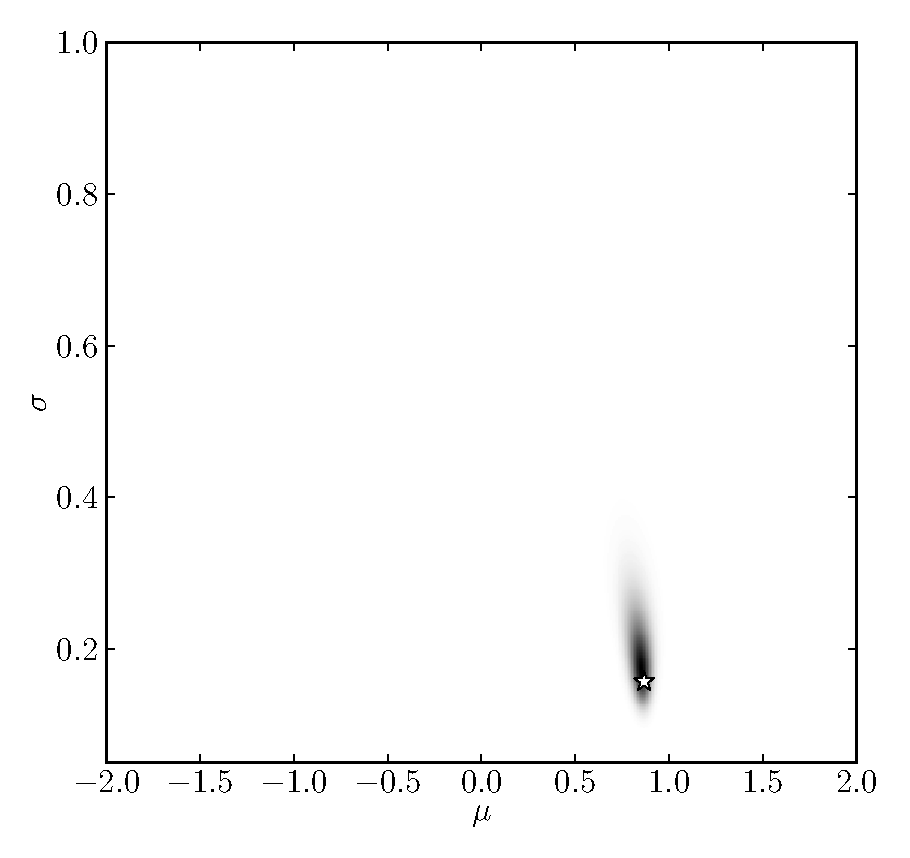
\includegraphics{Figures/posterior.eps}
\caption{\label{fig:posterior}}
\end{center}
\end{figure}



\section*{Acknowledgements}
It is a pleasure to thank Tommaso Treu, Anna Pancoast (UCSB), and
Brandon Kelly (UCSB) for many
useful conversations about reverberation mapping. The STAN team 



\begin{thebibliography}{99}
\bibitem[\protect\citeauthoryear{Barth et al.}{2013}]{2013ApJ...769..128B} 
Barth A.~J., et al., 2013, ApJ, 769, 128 

\bibitem[\protect\citeauthoryear{Bentz et al.}{2010}]{2010ApJ...720L..46B} 
Bentz M.~C., et al., 2010, ApJ, 720, L46 

\bibitem[\protect\citeauthoryear{Bovy Jo, Hogg, 
\& Roweis}{2011}]{extreme_deconvolution} Bovy Jo, Hogg D.~W., Roweis S.~T., 2011, AnApS, 5, 1657 

\bibitem[\protect\citeauthoryear{Brewer et al.}{2011}]{arp151} 
Brewer B.~J., et al., 2011, ApJ, 733, L33 

\bibitem[\protect\citeauthoryear{Brewer, P{\'a}rtay,
\& Cs{\'a}nyi}{2011}]{dnest} Brewer B.~J., P{\'a}rtay L.~B.,
Cs{\'a}nyi G., 2011, Statistics and Computing, 21, 4, 649-656. arXiv:0912.2380

\bibitem[\protect\citeauthoryear{Brewer, Foreman-Mackey, 
\& Hogg}{2013}]{2013AJ....146....7B} Brewer B.~J., Foreman-Mackey D., Hogg D.~W., 2013, AJ, 146, 7 

\bibitem[\protect\citeauthoryear{Fine et al.}{2013}]{2013MNRAS.434L..16F} 
Fine S., et al., 2013, MNRAS, 434, L16 

\bibitem[\protect\citeauthoryear{Fine et al.}{2012}]{2012MNRAS.427.2701F} 
Fine S., et al., 2012, MNRAS, 427, 2701 

\bibitem[\protect\citeauthoryear{Kelly}{2007}]{kelly} Kelly 
B.~C., 2007, ApJ, 665, 1489 

\bibitem[\protect\citeauthoryear{Kelly, Bechtold, 
\& Siemiginowska}{2009}]{2009ApJ...698..895K} Kelly B.~C., Bechtold J.,
Siemiginowska A., 2009, ApJ, 698, 895 

\bibitem[\protect\citeauthoryear{Krolik 
\& Done}{1995}]{1995ApJ...440..166K} Krolik J.~H., Done C., 1995, ApJ, 440, 166 

\bibitem[\protect\citeauthoryear{Loredo}{2004}]{loredo} Loredo 
T.~J., 2004, AIP Conference Series, 735, 195 

\bibitem[\protect\citeauthoryear{Loredo}{2012}]{2012arXiv1208.3036L} Loredo 
T.~J., 2012, arXiv, arXiv:1208.3036 

\bibitem[\protect\citeauthoryear{Hoffman 
\& Gelman}{2011}]{nuts} Hoffman M.~D., Gelman A., 2011, arXiv, arXiv:1111.4246 

\bibitem[\protect\citeauthoryear{Pancoast, Brewer, 
\& Treu}{2011}]{pancoast} Pancoast A., Brewer B.~J., Treu T., 2011, ApJ, 730, 139 

\bibitem[\protect\citeauthoryear{Zu et al.}{2013}]{2013ApJ...765..106Z} Zu 
Y., Kochanek C.~S., Koz{\l}owski S., Udalski A., 2013, ApJ, 765, 106 

\bibitem[\protect\citeauthoryear{Zu, Kochanek, 
\& Peterson}{2011}]{2011ApJ...735...80Z} Zu Y., Kochanek C.~S., Peterson B.~M., 2011, ApJ, 735, 80 



\end{thebibliography}



\end{document}

%%%%%%%%%%%%%%%%%%%%%%%%%%%%%%%%%%%%%%%%%%%%%%%%%%%%%%%%%%%%%%%%%%%%%%%%%%%%%%
